\documentclass{article}

% "preprint" shows the author name and a "Preprint." footer (no anonymous submission, no NeurIPS footer)
\usepackage[preprint]{neurips_2026}

\usepackage[utf8]{inputenc}
\usepackage[T1]{fontenc}
\usepackage{xcolor}
\definecolor{navy}{HTML}{123B5C}
\usepackage[colorlinks=true, linkcolor=navy, citecolor=navy, urlcolor=navy]{hyperref}
\usepackage{url}
\usepackage{booktabs}
\usepackage{amsfonts}
\usepackage{amsmath}
\usepackage{nicefrac}
\usepackage{microtype}
\usepackage{graphicx}
\usepackage{caption}
\usepackage{wrapfig}
\usepackage{float}
\captionsetup{font=small, skip=4pt}

% Tighter floats to stay within three pages
\setlength{\textfloatsep}{8pt plus 2pt minus 2pt}
\setlength{\floatsep}{6pt plus 2pt minus 2pt}
\setlength{\intextsep}{6pt plus 2pt minus 2pt}

% Same heading fonts as neurips_2026.sty, with less space around them
\makeatletter
\renewcommand{\section}{\@startsection{section}{1}{\z@}%
  {-1.4ex \@plus -0.3ex \@minus -0.2ex}{0.8ex \@plus 0.2ex}{\large\bf\raggedright}}
\renewcommand{\subsection}{\@startsection{subsection}{2}{\z@}%
  {-1.0ex \@plus -0.2ex \@minus -0.2ex}{0.3ex \@plus 0.1ex}{\normalsize\bf\raggedright}}
% Less space around the title rules
\renewcommand{\@toptitlebar}{\hrule height 4\p@ \vskip 0.15in \vskip -\parskip}
\renewcommand{\@bottomtitlebar}{\vskip 0.17in \vskip -\parskip \hrule height 1\p@ \vskip 0.05in}
% No "Preprint." footer; keep the two extra lines the style gives the first page
\renewcommand{\@notice}{\enlargethispage{2\baselineskip}}
\makeatother

\title{Trust in Automated Moderation of Toxic Comments\\
\large Milestone Report}

\author{%
  Martina Garc\'ia Gonz\'alez \\
  ECE 4424 / CS 4824 \\
  \href{https://github.com/martinagg7/ML-ToxicModeration}{Code repository} \quad
  \href{https://toxicmoderation.streamlit.app}{Live demo}
}

\begin{document}

\vspace*{-0.35in}
\maketitle
\vspace{-0.2in}

\begin{abstract}
Trust \& Safety teams often moderate comments with keyword blocklists that ignore context. On 1.8 million Jigsaw comments, we compare a blocklist and a TF-IDF model against DistilBERT, a contextual language model. DistilBERT achieves the highest F1 (0.67, against 0.61 and 0.15) and the lowest bias on comments that mention an identity. However, it still fails on negated insults and counter-speech, which motivates an abstention rule that defers uncertain cases to human review.
\end{abstract}
\vspace{-0.15in}

% ---------------------------------------------------------------
\section{Introduction}
\label{sec:intro}

\subsection{Requirement and question}
Trust \& Safety teams need to reduce manual review without systematic failures tied to the identity a comment mentions or to its phrasing, which a high average performance can hide~\citep{koh2021wilds}. We therefore ask when a toxicity classifier can decide autonomously, and when it should abstain in favour of human review.

\subsection{Revisions since the proposal}
The exploratory analysis showed that the \texttt{target} is the share of annotators who rated a comment as toxic, and that 33\% of toxic comments lie in the 0.4--0.6 band, where annotators disagree. We therefore trained DistilBERT on this continuous target (soft labels) to test whether it can reproduce this uncertainty. Since comments that mention an identity are more often toxic (Fig.~\ref{fig:toxic_identity}), errors on them also receive a higher weight in the loss.

\begin{figure}[H]
\centering
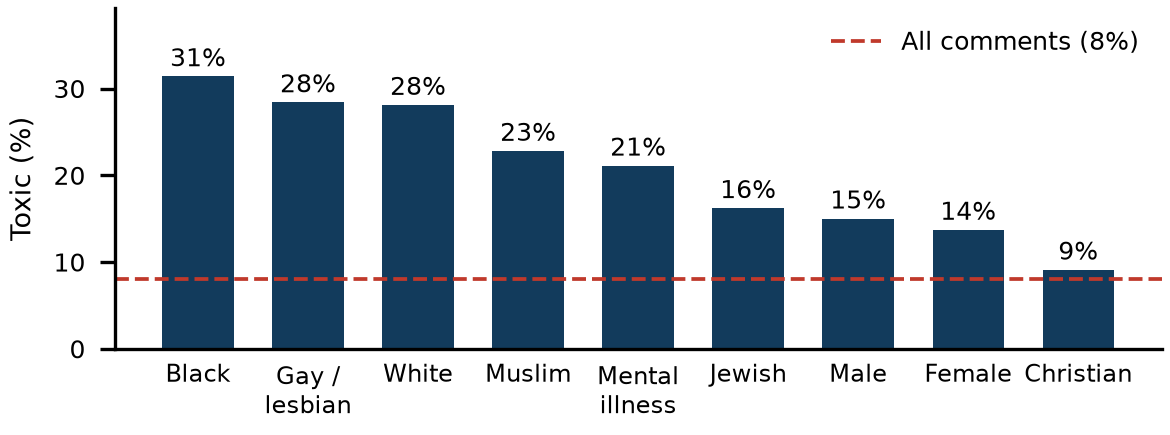
\includegraphics[width=0.6\linewidth]{figures/toxic_by_identity.png}
\caption{Share of toxic comments by identity mentioned in Jigsaw (dashed line: all comments, 8\%). A model can learn identity words as signals of toxicity.}
\label{fig:toxic_identity}
\end{figure}

\subsection{Current thesis}
\emph{DistilBERT moderates more accurately and with less identity bias than a blocklist or TF-IDF, but it is unreliable on disputed comments, identity mentions and negated insults. It should therefore decide alone only when its calibrated probability is conclusive.}

% ---------------------------------------------------------------
\section{Data and Evaluation Design}
\label{sec:data}

\subsection{Dataset and preprocessing}
We use the \href{https://www.kaggle.com/c/jigsaw-unintended-bias-in-toxicity-classification}{Jigsaw Unintended Bias} dataset~\citep{borkan2019nuanced}, with 1.8 million comments rated by a median of 4 annotators. A comment is toxic if its \texttt{target} is at least 0.5, which leaves only 8\% toxic comments. Nine identity groups are annotated in 22\% of the comments. After removing empty and duplicated comments, the data are split 80/10/10, stratified by label and grouped by article.

\subsection{Evaluation}
Models are compared with precision, recall and F1 at a threshold of 0.5, prioritising recall, since a published toxic comment is more costly than an extra review. Identity bias is measured with the false positive rate (FPR), the share of non-toxic comments wrongly blocked~\citep{dixon2018measuring}. We also designed 22 probe sentences with hard cases such as negations and counter-speech, a first test that \href{https://github.com/paul-rottger/hatecheck-data}{HateCheck}~\citep{rottger2021hatecheck} will extend.

% ---------------------------------------------------------------
\section{Methods}
\label{sec:methods}

\subsection{Blocklist}
As a representation of current practice, we use the public English \href{https://github.com/LDNOOBW/List-of-Dirty-Naughty-Obscene-and-Otherwise-Bad-Words}{LDNOOBW} list~\citep{ldnoobw} (403 terms) without modifications. A comment is blocked if it contains at least one of these terms as a whole word. Since the list has no parameters, it is evaluated directly on the test set.

\subsection{TF-IDF and logistic regression}
\begin{wrapfigure}{r}{0.4\linewidth}
\vspace{-14pt}
\centering
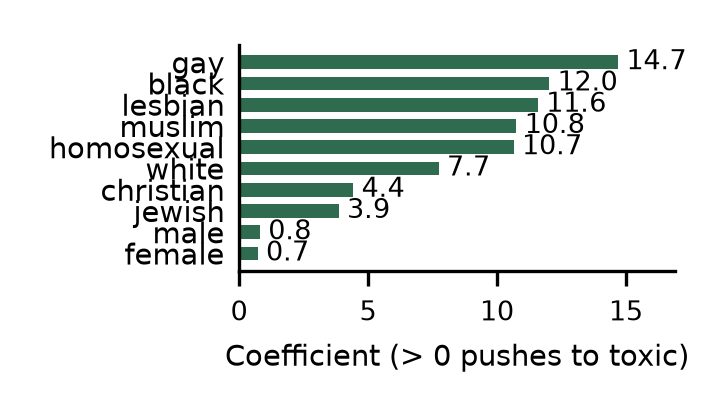
\includegraphics[width=\linewidth]{figures/tfidf_identity_weights.png}
\caption{TF-IDF coefficients of identity words.}
\label{fig:tfidf_weights}
\vspace{-12pt}
\end{wrapfigure}
Each comment is represented by the TF-IDF weights of its words and bigrams, that is, pairs of consecutive words. Bigrams allow an expression such as \emph{not bad} to receive a different weight from \emph{bad}. A logistic regression is then fitted on these vectors, with a regularisation coefficient $C=30$ selected on validation to avoid overfitting. All identity words receive positive coefficients, especially \emph{gay}, \emph{black} and \emph{lesbian} (Fig.~\ref{fig:tfidf_weights}), so their mere mention pushes a comment towards the toxic class.

\subsection{DistilBERT}
Comments are truncated to 128 tokens. \href{https://huggingface.co/distilbert/distilbert-base-uncased}{DistilBERT}~\citep{sanh2019distilbert} is a smaller version of BERT based on the Transformer architecture~\citep{alammar2018transformer}. It produces a contextual [CLS] vector that summarises the whole sentence~\citep{alammar2018bert}, and an MLP maps it to a probability of toxicity. The model is fine-tuned following the Hugging Face text classification guide~\citep{huggingface2024textclass}. We tested several training configurations (Table~\ref{tab:dev}), including binary labels, soft labels, and soft labels with a higher loss weight for comments that mention an identity (3 for non-toxic and 2 for toxic ones, against 1 for the rest). The final model uses this last configuration, trained for 2 epochs with a learning rate of $2\times10^{-5}$ and selected by validation PR-AUC. Training was done on a single NVIDIA RTX 5060 GPU, at about 100 minutes per run.

% ---------------------------------------------------------------
\section{Preliminary Results}
\label{sec:results}

\subsection{Overall performance}
\noindent
\begin{minipage}[c]{0.5\linewidth}
DistilBERT outperforms both baselines on every metric (Table~\ref{tab:test}). The blocklist detects only 10\% of toxic comments, since its list contains mostly sexual vocabulary, while the most frequent insults in Jigsaw are words such as \emph{idiot} or \emph{stupid}. Recall remains the main weakness, as DistilBERT still misses 42\% of toxic comments.
\end{minipage}\hfill
\begin{minipage}[c]{0.46\linewidth}
\centering
\footnotesize
\setlength{\tabcolsep}{4pt}
\begin{tabular}{lcccc}
\toprule
Model & Prec. & Rec. & F1 & FPR \\
\midrule
Blocklist   & 0.27 & 0.10 & 0.15 & 2.3\% \\
TF-IDF + LR & 0.73 & 0.53 & 0.61 & 1.7\% \\
DistilBERT  & \textbf{0.80} & \textbf{0.58} & \textbf{0.67} & \textbf{1.3\%} \\
\bottomrule
\end{tabular}
\captionof{table}{Test results (threshold 0.5).}
\label{tab:test}
\end{minipage}

\subsection{Development runs and failed attempts}
\noindent
\begin{minipage}[c]{0.5\linewidth}
Freezing the encoder and training only the MLP performs worse than TF-IDF. With binary labels, the model overfits after the second epoch. Soft labels give the largest improvement, while identity weights do not improve the global metrics but slightly reduce the FPR on identity groups (Table~\ref{tab:dev}).
\end{minipage}\hfill
\begin{minipage}[c]{0.46\linewidth}
\centering
\footnotesize
\setlength{\tabcolsep}{4pt}
\begin{tabular}{lcc}
\toprule
Configuration & PR-AUC & F1 \\
\midrule
Frozen encoder          & 0.486 & 0.309 \\
Binary labels           & 0.767 & 0.645 \\
Soft labels             & \textbf{0.790} & 0.679 \\
Soft + identity weights & 0.788 & 0.679 \\
\bottomrule
\end{tabular}
\captionof{table}{DistilBERT on validation (final: last row).}
\label{tab:dev}
\end{minipage}

\subsection{Identity bias}
All three models wrongly block comments that mention an identity more often than average (Fig.~\ref{fig:fpr}). The blocklist fails mostly on gender and sexual orientation, and TF-IDF on race and religion. DistilBERT has the lowest FPR in 8 of the 9 groups, but its bias is reduced rather than removed, reaching 5.6\% for gay or lesbian and 5.4\% for Black, against 1.3\% overall.

\begin{figure}[H]
\centering
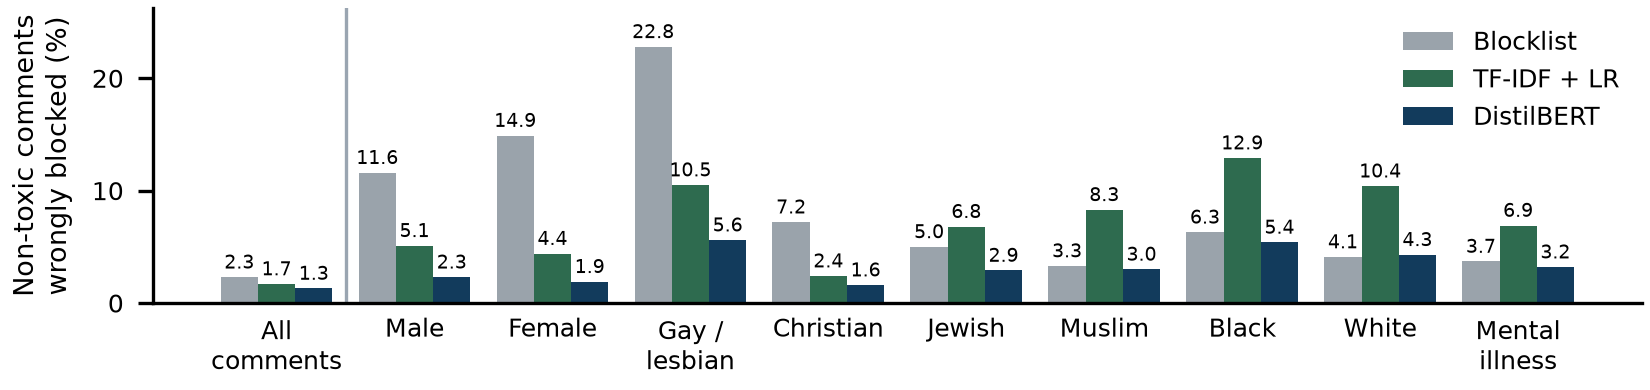
\includegraphics[width=\linewidth]{figures/fpr_by_identity.png}
\caption{FPR by identity group (test).}
\label{fig:fpr}
\end{figure}

\subsection{Annotator disagreement}
\noindent
\begin{minipage}[t]{0.6\linewidth}
\vspace{0pt}
Errors concentrate on disputed comments. In the 0.4--0.6 band, DistilBERT misclassifies 38\% of comments, against 0.7\% of clearly non-toxic ones. In this band, DistilBERT gives intermediate probabilities, while TF-IDF pushes them towards 0 (Fig.~\ref{fig:bands}). This suggests that soft labels help the model reproduce annotator uncertainty, which is the basis for the planned abstention rule.
\end{minipage}\hfill
\begin{minipage}[t]{0.36\linewidth}
\vspace{0pt}
\centering
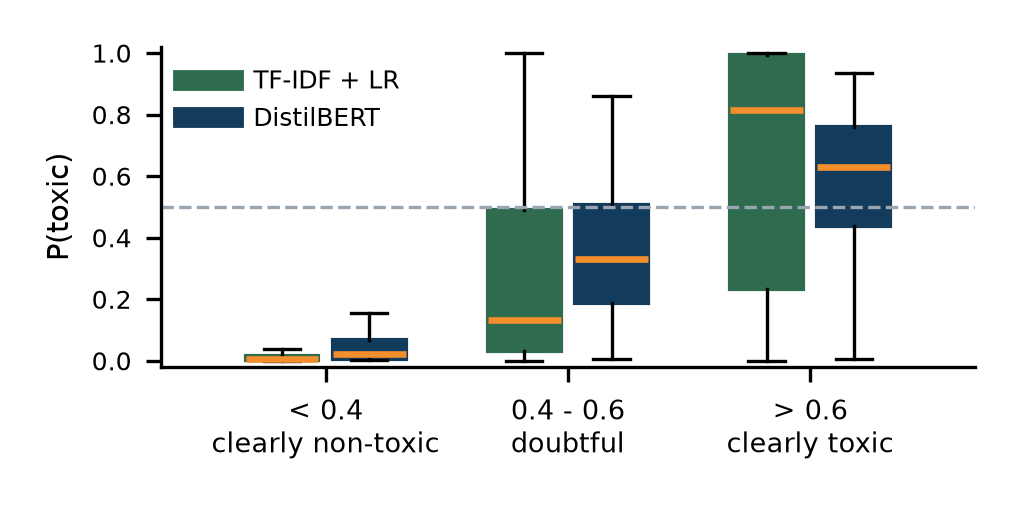
\includegraphics[width=\linewidth]{figures/prob_by_band.png}
\captionof{figure}{Predicted probability by target band.}
\label{fig:bands}
\end{minipage}

\subsection{What the evidence supports}
The evidence supports that DistilBERT outperforms both baselines, but not that it can moderate autonomously, since it misses 42\% of toxic comments and over-blocks some identity groups. On the probes, it handles \emph{``I don't hate gay people''} but still blocks \emph{``You are not an idiot''} and \emph{``My neighbor is black''}. Results come from a single seed and data source, so small differences should be read with caution.

% ---------------------------------------------------------------
\section{Next Steps, Class Survey and Contributions}
\label{sec:next}

\subsection{Next test and completion plan}
The next test is HateCheck, with hard cases such as negation, counter-speech and reclaimed slurs outside the Jigsaw distribution. We will then calibrate DistilBERT with temperature scaling~\citep{guo2017calibration}, measure its ECE and define the abstention rule. Since GPU time is the main risk, these steps only use saved predictions and need no retraining.

\subsection{Class-survey case summary}
This is an uncertainty case. DistilBERT is better on average but unreliable for some groups and doubtful comments, which raises the question of whether a biased model can be used ethically if a human reviews its doubtful decisions.

\begin{table}[H]
\centering
\footnotesize
\begin{tabular}{@{}p{0.25\linewidth}p{0.7\linewidth}@{}}
\toprule
Domain / decision & Trust \& Safety, publish, block or review \\
Evidence / baseline & Jigsaw (1.8\,M comments), keyword blocklist and TF-IDF \\
Stress condition & Identity groups, annotator disagreement, HateCheck \\
Uncertainty handling & Abstain when the calibrated probability is uncertain \\
Supported claim & Better than current practice, not reliable without human review \\
\bottomrule
\end{tabular}
\caption{Draft comparison-matrix entry.}
\label{tab:matrix}
\end{table}

\noindent\textbf{Contributions.} Martina Garc\'ia Gonz\'alez (sole author) carried out all parts of this project.

% References do not count towards the page limit
\small
\bibliographystyle{plainnat}
\bibliography{references}

\end{document}
